%File: formatting-instruction.tex
\documentclass[letterpaper]{article}
\usepackage{aaai}
\usepackage{times}
\usepackage{helvet}
\usepackage{courier}
\usepackage{graphicx}
\usepackage{xcolor}
\usepackage{natbib}
\bibliographystyle{aaai}
% Sudo Code packages
\usepackage[ruled, linesnumbered]{algorithm2e}

\usepackage{amsfonts}

\graphicspath{../../}

\frenchspacing
\setlength{\pdfpagewidth}{8.5in}
\setlength{\pdfpageheight}{11in}
\pdfinfo{
/Title (Reinforcement Learning: Parking lot)
/Author (Robert Horton)}
\setcounter{secnumdepth}{0}  
 \begin{document}

% The file aaai.sty is the style file for AAAI Press 
% proceedings, working notes, and technical reports.
%
\title{Reinforcement Learning\\ Artificial Neural Network: Valet Parking Lot }
\author{Robert Horton\\
UCCS\\
1420 Austin Bluffs Pkwy,\\
Colorado Springs, Colorado 80918\\
}
\maketitle

% ----------------------------------------------- Abstract
\begin{abstract}
\begin{quote}
In society when considering segregation amongst several different groups there seems to be just as many physiological phenomenons as there are seemingly counter intuitive revelations.Through coded implementation, an instance of a randomly generated  graph can be generated to run \textit{contentedness}.  With varying parameter values, we analyse dynamic graph interactions amongst agents in a society with spatial awareness of neighbours within a set distance of direct neighbours.   
\end{quote}
\end{abstract}

% ----------------------------------------------- Introduction
\section{Introduction}

Deliv: 01:\\
In the PDF, provide several examples (for example, using small 3x3 or 4x4 grids) to verify that your “contentedness” and “move-to-empty” functions are operating as intended. Also note: step 2 in the algorithm above is ambiguous (i.e., I didn’t tell you whether to iterate over the grid, over the agents, or in what order; I also didn’t tell you whether to check satisfaction for all agents before moving any, or if you should check- move check-move one-by-one). Your PDF should explain precisely and explicitly how you decided to resolve this ambiguity! I.e., give a precise description of your satisfaction-checking and agent-moving mechanic.\\ \\
Deliv: 02:\\
How segregated is the map throughout a simulation run? Create a function which checks the cross-type-fraction (CTF) of a snapshot of the map. As demonstrated in class, this function will divide the number of different-type neighbors (summed over all agents) by the total number of neighbors (summed over all agents). You should be able to call your function at each step along a simulation to see how the CTF changes as agents move around.\\\\
Create a series of plots which demonstrate how the CTF changes over the course of several simulation runs of the model. Each plot should have iteration number on the horizontal axis. You should choose at least 3 sets of parameter values (i.e., at least 3 differentcombinations red/blue split, satisfaction threshold t, and \% empty). For each of these 3 sets of parameter values, do 5-10 simulation runs and plot their CTF traces together. You should have one plot with 5-10 traces for each of the 3 sets of parameter values, for a total of 3 plots. Clearly mark what parameter values gave rise to each of the plots. 3. How does segregation depend on parameter values? Create a function which measures the average CTF at the end of a simulation run as a function of input parameters. Your function’s call signature should be average CTF(red blue split, t, pct empty) When called, this function should perform 10 simulation runs with those parameters, record the CTF found at the end of each run, and then return the average of those 10 CTF values.  

\begin{center}
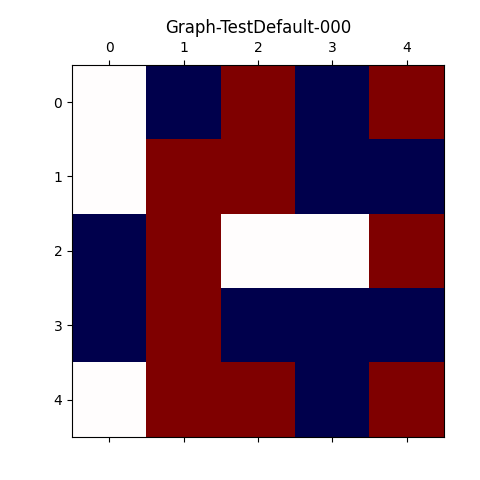
\includegraphics[scale=0.7]{./Content/GeneratedGraphs/Graph-TestDefault-0.1-0.5-0.2/Graph-TestDefault-000}
\end{center}

% ----------------------------------------------- Implementation
\section{Implementation}  

Book for the class  (\cite{10.5555/1805895})\\
web site for python (\cite{AdilMoujahid})\\
paper for segregation with graphs (\cite{ijcai2019-38})\\

% ----------------------- Execution 
\subsection{Execution}

% ----------------------- Analyisis 
\subsection{Analyisis}
 
% ----------------------------------------------- Conclusion
\section{Conclusion}

% ----------------------------------------------- References 

\bibliography{ArticleTemplate}

\end{document}